\chapter{The Elder Heliosystem: A Unified Closed System}

\section{System Overview and Core Principles}

The Elder Heliosystem represents a comprehensive mathematical framework for hierarchical knowledge representation and learning, designed as a fully integrated closed system. Unlike traditional learning systems that operate on flat parameter spaces, the Elder Heliosystem organizes knowledge in concentric heliomorphic shells with complex-valued parameters that encode both magnitude and phase information.

\begin{definition}[Elder Heliosystem]
The Elder Heliosystem is a triple $(\mathcal{E}, \mathcal{M}, \mathcal{E}r)$ where:
\begin{itemize}
    \item $\mathcal{E}$ is the Elder entity, responsible for universal principles across domains
    \item $\mathcal{M}$ is a set of Mentor entities $\{\mathcal{M}_1, \mathcal{M}_2, \ldots, \mathcal{M}_M\}$, each specialized in a specific domain
    \item $\mathcal{E}r$ is a collection of Erudite entities $\{\mathcal{E}r_{i,j}\}_{i=1,j=1}^{M,N_i}$, where each $\mathcal{E}r_{i,j}$ is responsible for a specific task $j$ in domain $i$
\end{itemize}
\end{definition}

The system's foundation rests on three key principles that distinguish it from traditional learning architectures:

\begin{enumerate}
    \item \textbf{Heliomorphic Structure}: Knowledge is organized in concentric shells radiating from a central core, creating a nested hierarchy where inner shells influence outer shells through resonance patterns.
    
    \item \textbf{Complex-Valued Representation}: Parameters $\theta \in \complexn{d}$ are represented as complex numbers $\theta = \rho e^{i\phi}$, where magnitude $\rho$ encodes parameter importance and phase $\phi$ encodes parameter alignment.
    
    \item \textbf{Orbital Dynamics}: Knowledge transfer between entities follows orbital mechanics, where the Elder acts as the "sun," Mentors as "planets," and Erudites as "moons," creating a gravitational system of influence.
\end{enumerate}

\section{Hierarchical Knowledge Flow in the Closed System}

The Elder Heliosystem operates as a fully closed system with bidirectional knowledge flow:

\begin{figure}[h]
\centering
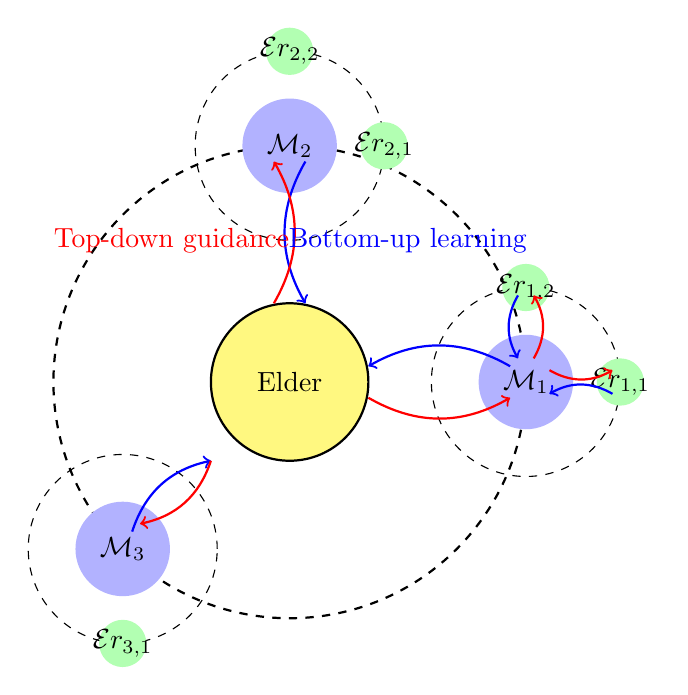
\begin{tikzpicture}[node distance=2.5cm, thick]
    % Draw the Elder as the sun
    \draw[fill=yellow!50] (0,0) circle (1cm);
    \node at (0,0) {Elder};
    
    % Draw the Mentor orbits and planets
    \draw[dashed] (0,0) circle (3cm);
    \fill[blue!30] (3,0) circle (0.6cm);
    \node at (3,0) {$\mathcal{M}_1$};
    \fill[blue!30] (0,3) circle (0.6cm);
    \node at (0,3) {$\mathcal{M}_2$};
    \fill[blue!30] (-2.12,-2.12) circle (0.6cm);
    \node at (-2.12,-2.12) {$\mathcal{M}_3$};
    
    % Draw Erudite orbits and moons for M1
    \draw[dashed, thin] (3,0) circle (1.2cm);
    \fill[green!30] (4.2,0) circle (0.3cm);
    \node at (4.2,0) {$\mathcal{E}r_{1,1}$};
    \fill[green!30] (3,1.2) circle (0.3cm);
    \node at (3,1.2) {$\mathcal{E}r_{1,2}$};
    
    % Draw Erudite orbits and moons for M2
    \draw[dashed, thin] (0,3) circle (1.2cm);
    \fill[green!30] (1.2,3) circle (0.3cm);
    \node at (1.2,3) {$\mathcal{E}r_{2,1}$};
    \fill[green!30] (0,4.2) circle (0.3cm);
    \node at (0,4.2) {$\mathcal{E}r_{2,2}$};
    
    % Draw Erudite orbits and moons for M3
    \draw[dashed, thin] (-2.12,-2.12) circle (1.2cm);
    \fill[green!30] (-2.12,-3.32) circle (0.3cm);
    \node at (-2.12,-3.32) {$\mathcal{E}r_{3,1}$};
    
    % Draw arrows for knowledge flow
    % Bottom-up flow (from Erudite to Mentor)
    \draw[->, blue, thick] (4.1,-0.15) to[bend right] (3.3,-0.15);
    \draw[->, blue, thick] (2.9,1.1) to[bend right] (2.9,0.3);
    
    % Bottom-up flow (from Mentor to Elder)
    \draw[->, blue, thick] (2.8,0.2) to[bend right] (1.0,0.2);
    \draw[->, blue, thick] (0.2,2.8) to[bend right] (0.2,1.0);
    \draw[->, blue, thick] (-2.0,-1.9) to[bend left] (-1.0,-1.0);
    
    % Top-down flow (from Elder to Mentor)
    \draw[->, red, thick] (1.0,-0.2) to[bend right] (2.8,-0.2);
    \draw[->, red, thick] (-0.2,1.0) to[bend right] (-0.2,2.8);
    \draw[->, red, thick] (-1.0,-1.0) to[bend left] (-1.9,-1.8);
    
    % Top-down flow (from Mentor to Erudite)
    \draw[->, red, thick] (3.3,0.15) to[bend right] (4.1,0.15);
    \draw[->, red, thick] (3.1,0.3) to[bend right] (3.1,1.1);
    
    % Label the flows
    \node[blue] at (1.5,1.8) {Bottom-up learning};
    \node[red] at (-1.5,1.8) {Top-down guidance};
\end{tikzpicture}
\caption{Bidirectional knowledge flow in the Elder Heliosystem}
\label{fig:knowledge_flow}
\end{figure}

The knowledge flow occurs through two primary mechanisms:

\begin{enumerate}
    \item \textbf{Bottom-up Learning}: Domain-specific knowledge from Erudites flows up to their respective Mentors, which extract domain-level meta-knowledge. This meta-knowledge then flows to the Elder, which identifies universal principles applicable across domains.
    
    \item \textbf{Top-down Guidance}: Universal principles discovered by the Elder flow down to Mentors, providing cross-domain insights that guide domain-specific learning. Mentors then adapt these principles to their specific domains and guide their Erudites accordingly.
\end{enumerate}

\section{Complex-Valued Parameter Representation}

A fundamental aspect of the Elder Heliosystem's closed operation is the complex-valued parameter representation, which encodes both magnitude and phase information:

\begin{equation}
\theta = \rho e^{i\phi} \in \complexn{d}
\end{equation}

Where:
\begin{itemize}
    \item $\rho \in \mathbb{R}^+$ is the magnitude, representing parameter importance
    \item $\phi \in [0, 2\pi)$ is the phase, representing parameter alignment
    \item $d$ is the dimensionality of the parameter space
\end{itemize}

This representation enables three critical capabilities that maintain system coherence:

\begin{enumerate}
    \item \textbf{Phase Coherence}: Parameters with aligned phases (similar $\phi$ values) work together coherently, reducing effective dimensionality and creating structured learning.
    
    \item \textbf{Magnitude-Based Pruning}: Parameters with small magnitudes $\rho$ contribute minimally and can be pruned, creating an automatic dimensionality reduction.
    
    \item \textbf{Rotational Dynamics}: Knowledge transfer between entities operates through phase rotations, preserving energy while redistributing information.
\end{enumerate}

The complex-valued structure creates a self-regulating system where parameter interactions automatically adjust to maintain system stability and coherence.

\section{Heliomorphic Shells and Manifold Structure}

The Elder Heliosystem organizes knowledge in concentric heliomorphic shells, creating a structured manifold that constrains parameter evolution:

\begin{equation}
\mathcal{H}_n = \{\theta \in \complexn{d} \mid \|\theta\|_{\helio} = r_n\}
\end{equation}

Where $\mathcal{H}_n$ is the $n$-th heliomorphic shell with radius $r_n$, and $\|\cdot\|_{\helio}$ is the heliomorphic norm.

This shell structure creates natural boundaries for different types of knowledge:

\begin{itemize}
    \item \textbf{Inner Shell} ($\mathcal{H}_1$): Contains Elder parameters representing universal principles
    \item \textbf{Middle Shells} ($\mathcal{H}_2, \ldots, \mathcal{H}_{M+1}$): Contain Mentor parameters for domain-specific meta-knowledge
    \item \textbf{Outer Shells} ($\mathcal{H}_{M+2}, \ldots$): Contain Erudite parameters for task-specific knowledge
\end{itemize}

As learning progresses, parameters naturally self-organize into these shells, creating an emergent hierarchical structure without explicit architectural constraints.

\section{Orbital Resonance and Knowledge Transfer}

The Elder Heliosystem's closed nature is maintained through orbital resonance, where entities in different shells synchronize their learning through phase-locked relationships:

\begin{equation}
n\omega_{\text{Elder}} = m\omega_{\text{Mentor}} = k\omega_{\text{Erudite}}
\end{equation}

Where $\omega_{\text{Elder}}$, $\omega_{\text{Mentor}}$, and $\omega_{\text{Erudite}}$ are the orbital frequencies of parameters in their respective shells, and $n$, $m$, and $k$ are small integers.

This resonance mechanism enables efficient knowledge transfer with minimal parameter exchange through:

\begin{enumerate}
    \item \textbf{Mean Motion Resonance}: Periodic alignment of parameters between shells creates windows for efficient knowledge transfer.
    
    \item \textbf{Spin-Orbit Coupling}: Phase relationships between parameter rotation and orbital motion stabilize learning trajectories.
    
    \item \textbf{Resonance Bandwidth}: Tolerance ranges around exact resonance ratios allow flexible adaptation while maintaining system stability.
\end{enumerate}

\section{The Unified Learning Process}

The complete learning process in the Elder Heliosystem operates through a unified algorithm that maintains system closure:

\begin{algorithm}
\caption{Elder Heliosystem Unified Learning}
\begin{algorithmic}[1]
\State \textbf{Input:} Domain datasets $\{\mathcal{D}_i\}_{i=1}^M$, initial parameters 
\State \textbf{Output:} Trained Elder, Mentor, and Erudite parameters

\State \textit{// Initialize the heliomorphic shells}
\State $\mathcal{H}_{\text{Elder}} \gets \{\theta \in \complexn{d_E} \mid \|\theta\|_{\helio} = r_{\text{Elder}}\}$
\State $\mathcal{H}_{\text{Mentor}} \gets \{\theta \in \complexn{d_M} \mid \|\theta\|_{\helio} = r_{\text{Mentor}}\}$
\State $\mathcal{H}_{\text{Erudite}} \gets \{\theta \in \complexn{d_E} \mid \|\theta\|_{\helio} = r_{\text{Erudite}}\}$

\For{each training epoch}
    \State \textit{// Bottom-up learning phase}
    \For{each domain $\mathcal{D}_i$}
        \For{each task $j$ in domain $\mathcal{D}_i$}
            \State Update Erudite parameters $\theta_{\text{E},i,j}$ using task-specific data
            \State Project updated parameters back onto $\mathcal{H}_{\text{Erudite}}$
        \EndFor
        \State Aggregate knowledge from Erudites to update Mentor parameters $\theta_{\text{M},i}$
        \State Project updated parameters back onto $\mathcal{H}_{\text{Mentor}}$
    \EndFor
    \State Aggregate knowledge from Mentors to update Elder parameters $\theta_{\text{Elder}}$
    \State Project updated parameters back onto $\mathcal{H}_{\text{Elder}}$
    
    \State \textit{// Orbital resonance harmonization}
    \State Adjust orbital frequencies to maintain $n\omega_{\text{Elder}} = m\omega_{\text{Mentor}} = k\omega_{\text{Erudite}}$
    
    \State \textit{// Top-down guidance phase}
    \State Propagate universal principles from Elder to all Mentors
    \State Propagate domain-specific knowledge from each Mentor to its Erudites
\EndFor
\end{algorithmic}
\end{algorithm}

This unified algorithm ensures that:

\begin{enumerate}
    \item Knowledge flows bidirectionally between levels
    \item Parameters remain confined to their appropriate heliomorphic shells
    \item Orbital resonance maintains system coherence
    \item Phase coherence enables efficient learning with reduced effective dimensionality
\end{enumerate}

\section{Gradient Flow on the Heliomorphic Manifold}

The Elder Heliosystem achieves stable learning through specialized gradient flow on the heliomorphic manifold:

\begin{equation}
\frac{d\theta}{dt} = -\helioderiv \mathcal{L}(\theta)
\end{equation}

Where $\helioderiv$ is the heliomorphic gradient operator that respects the manifold's structure.

This gradient flow has three key properties that maintain system closure:

\begin{enumerate}
    \item \textbf{Shell Preservation}: Updates keep parameters on their respective shells, maintaining the hierarchical structure.
    
    \item \textbf{Phase-Amplitude Separation}: Gradient updates separately modify phase and amplitude components, allowing finer control over knowledge evolution.
    
    \item \textbf{Geodesic Motion}: Parameters follow geodesic paths on the heliomorphic manifold rather than straight-line Euclidean paths, preserving the system's geometric constraints.
\end{enumerate}

\section{Energy Conservation and Self-Regulation}

As a closed system, the Elder Heliosystem maintains energy conservation principles that enable self-regulation:

\begin{equation}
E_{\text{total}} = E_{\text{Elder}} + \sum_{i=1}^M E_{\text{Mentor},i} + \sum_{i=1}^M \sum_{j=1}^{N_i} E_{\text{Erudite},i,j} = \text{constant}
\end{equation}

Where $E_{\text{Elder}}$, $E_{\text{Mentor},i}$, and $E_{\text{Erudite},i,j}$ represent the energy (complexity) of parameters at each level.

This energy conservation principle creates several self-regulating properties:

\begin{enumerate}
    \item \textbf{Automatic Complexity Control}: The system naturally distributes complexity across levels, preventing any single component from becoming unnecessarily complex.
    
    \item \textbf{Knowledge Condensation}: Universal patterns migrate to inner shells, reducing redundancy and creating compact representations.
    
    \item \textbf{Adaptive Learning Rates}: Orbital dynamics naturally adjust learning rates based on current knowledge state, accelerating in sparse knowledge regions and decelerating in dense regions.
\end{enumerate}

\section{Cross-Domain Knowledge Transfer}

A crucial feature of the Elder Heliosystem as a closed system is its ability to transfer knowledge across domains through the Elder entity:

\begin{equation}
\mathcal{T}(D_i \rightarrow D_j) = \helioexp_{\theta_{\text{M},j}}(\helioderiv \theta_{\text{Elder}}(\helioderiv \theta_{\text{M},i}))
\end{equation}

Where $\mathcal{T}(D_i \rightarrow D_j)$ represents knowledge transfer from domain $D_i$ to domain $D_j$, and $\helioexp$ is the heliomorphic exponential map.

This transfer mechanism operates entirely within the closed system without external components, creating:

\begin{enumerate}
    \item \textbf{Zero-Shot Transfer}: The ability to apply knowledge to entirely new domains without specific training.
    
    \item \textbf{Resonance-Boosted Learning}: New domains aligned with existing knowledge experience accelerated learning through resonance effects.
    
    \item \textbf{Domain Alignment}: The phase component of complex parameters automatically aligns related concepts across domains.
\end{enumerate}

\section{Practical Implementation and System Completeness}

The Elder Heliosystem's implementation relies on a complete set of mathematical kernels organized in a dependency hierarchy:

\begin{figure}[h]
\centering
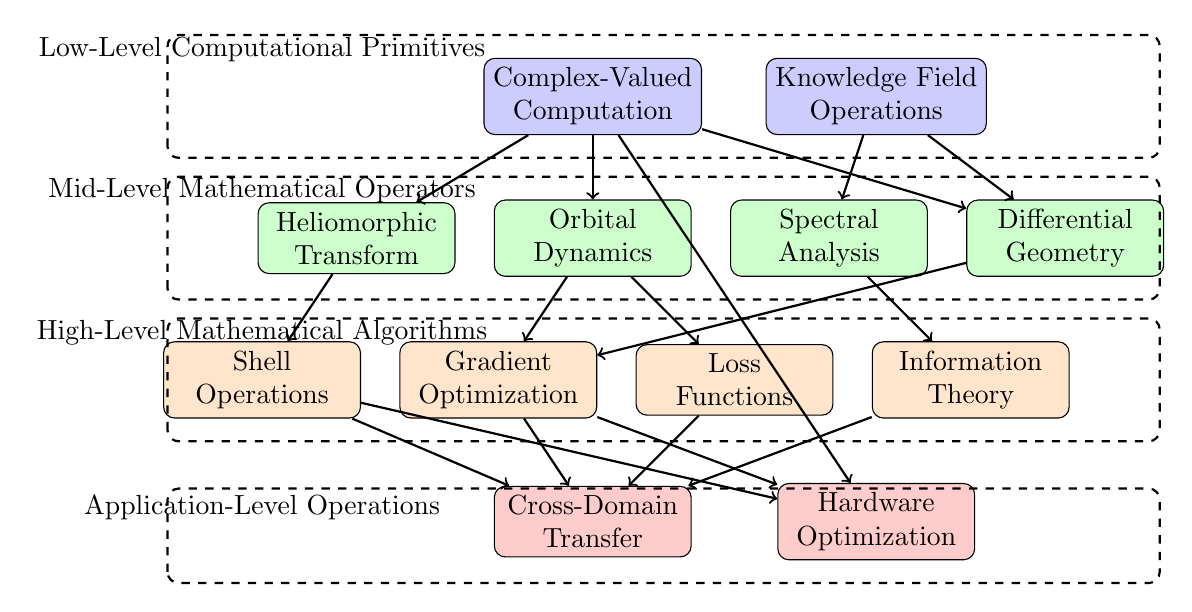
\begin{tikzpicture}[scale=0.6]
    % Define basic node style
    \tikzset{
        block/.style={
            rectangle,
            rounded corners,
            draw,
            minimum width=2.5cm,
            minimum height=0.8cm,
            align=center
        }
    }
    
    % Low-level kernels (blue)
    \node[block, fill=blue!20] (complex) at (0,8) {Complex-Valued\\Computation};
    \node[block, fill=blue!20] (field) at (6,8) {Knowledge Field\\Operations};
    
    % Mid-level kernels (green)
    \node[block, fill=green!20] (helio) at (-5,5) {Heliomorphic\\Transform};
    \node[block, fill=green!20] (orbital) at (0,5) {Orbital\\Dynamics};
    \node[block, fill=green!20] (spectral) at (5,5) {Spectral\\Analysis};
    \node[block, fill=green!20] (geometry) at (10,5) {Differential\\Geometry};
    
    % High-level kernels (orange)
    \node[block, fill=orange!20] (shell) at (-7,2) {Shell\\Operations};
    \node[block, fill=orange!20] (gradient) at (-2,2) {Gradient\\Optimization};
    \node[block, fill=orange!20] (loss) at (3,2) {Loss\\Functions};
    \node[block, fill=orange!20] (info) at (8,2) {Information\\Theory};
    
    % Application-level kernels (red)
    \node[block, fill=red!20] (transfer) at (0,-1) {Cross-Domain\\Transfer};
    \node[block, fill=red!20] (hardware) at (6,-1) {Hardware\\Optimization};
    
    % Connections between low-level and mid-level
    \draw[->, thick] (complex) -- (helio);
    \draw[->, thick] (complex) -- (orbital);
    \draw[->, thick] (field) -- (spectral);
    \draw[->, thick] (field) -- (geometry);
    \draw[->, thick] (complex) -- (geometry);
    
    % Connections between mid-level and high-level
    \draw[->, thick] (helio) -- (shell);
    \draw[->, thick] (orbital) -- (gradient);
    \draw[->, thick] (orbital) -- (loss);
    \draw[->, thick] (spectral) -- (info);
    \draw[->, thick] (geometry) -- (gradient);
    
    % Connections to application level
    \draw[->, thick] (shell) -- (transfer);
    \draw[->, thick] (gradient) -- (transfer);
    \draw[->, thick] (loss) -- (transfer);
    \draw[->, thick] (info) -- (transfer);
    
    \draw[->, thick] (shell) -- (hardware);
    \draw[->, thick] (gradient) -- (hardware);
    \draw[->, thick] (complex) -- (hardware);
    
    % Layer boundaries
    \draw[dashed, rounded corners, thick] (-9,6.7) rectangle (12,9.3);
    \node at (-7,9) {Low-Level Computational Primitives};
    
    \draw[dashed, rounded corners, thick] (-9,3.7) rectangle (12,6.3);
    \node at (-7,6) {Mid-Level Mathematical Operators};
    
    \draw[dashed, rounded corners, thick] (-9,0.7) rectangle (12,3.3);
    \node at (-7,3) {High-Level Mathematical Algorithms};
    
    \draw[dashed, rounded corners, thick] (-9,-2.3) rectangle (12,-0.3);
    \node at (-7,-0.7) {Application-Level Operations};
\end{tikzpicture}
\caption{Kernel dependency hierarchy for the Elder Heliosystem implementation}
\label{fig:kernel_dependencies}
\end{figure}

This complete set of mathematical kernels enables the Elder Heliosystem to operate as a fully self-contained, closed system that:

\begin{enumerate}
    \item Extracts universal principles across domains (Elder level)
    \item Accumulates meta-knowledge within domains (Mentor level)
    \item Learns specific tasks in each domain (Erudite level)
    \item Transfers knowledge between domains through principled mathematical operations
    \item Self-organizes parameters into heliomorphic shells
    \item Maintains system coherence through orbital resonance
\end{enumerate}

\section{System-Determined Parameter Sparsity}

A critical feature of the Elder Heliosystem is its dynamic control of parameter activation through system-determined sparsity. Unlike traditional neural networks that utilize fixed sparsity patterns or manually-tuned dropout rates, the Elder Heliosystem employs emergent sparsity governed by the current state of the system itself.

\subsection{Sparsity Factor Determination}

The system's parameter activation is governed by a sparsity factor $\sigma$ that emerges from the interplay of multiple system states:

\begin{equation}
\sigma = \sigma_{\text{base}} \cdot f_{\text{phase}}(\Phi) \cdot f_{\text{harmony}}(\Omega) \cdot f_{\text{cyclical}}(\phi_E)
\end{equation}

Where:
\begin{itemize}
    \item $\sigma_{\text{base}} \approx 10^{-4}$ is the baseline sparsity factor (0.01\%)
    \item $f_{\text{phase}}(\Phi)$ is the phase concentration modulation function
    \item $f_{\text{harmony}}(\Omega)$ is the orbital harmony modulation function
    \item $f_{\text{cyclical}}(\phi_E)$ introduces intentional cyclical patterns based on Elder phase
\end{itemize}

\subsection{Phase Concentration Factor}

The phase concentration factor measures how concentrated the Mentor entities are around the Elder in phase space:

\begin{equation}
f_{\text{phase}}(\Phi) = \gamma_{\text{phase}} + (1 - \gamma_{\text{phase}})(1 - C(\Phi))
\end{equation}

Where $C(\Phi)$ is the concentration metric for the set of phase differences $\Phi = \{\phi_M - \phi_E \mid M \in \mathcal{M}\}$ between all Mentors and the Elder, and $\gamma_{\text{phase}} \approx 0.4$ is a weighting constant.

When Mentors have phases closely aligned with the Elder (high concentration), the system becomes more selective in parameter activation, reducing sparsity. Conversely, when Mentors are dispersed in phase space, the system activates a broader parameter set.

\subsection{Orbital Harmony Factor}

The orbital harmony factor assesses the regularity of orbital positions through phase quadrant distribution:

\begin{equation}
f_{\text{harmony}}(\Omega) = \gamma_{\text{harmony}} + (1 - \gamma_{\text{harmony}})H(\Omega)
\end{equation}

Where $H(\Omega)$ is the harmony metric for the orbital configuration $\Omega$, measured as the inverse of normalized variance in quadrant population, and $\gamma_{\text{harmony}} \approx 0.4$ is a weighting constant.

Higher orbital harmony (more balanced distribution across phase quadrants) leads to increased parameter activation, as the system can utilize more structured activation patterns. This creates efficient parameter sharing across different orbital regions.

\subsection{Cyclical Component}

The Elder entity introduces intentional cyclical patterns in parameter activation:

\begin{equation}
f_{\text{cyclical}}(\phi_E) = \gamma_{\text{cycle}} + (1 - \gamma_{\text{cycle}})(0.5 + 0.5\sin(k\phi_E))
\end{equation}

Where $\phi_E$ is the Elder phase, $k \approx 3$ is a frequency multiplier, and $\gamma_{\text{cycle}} \approx 0.4$ is a weighting constant.

This cyclical pattern creates structured variation in memory usage over time, allowing the system to allocate processing resources differently during different phases of operation.

\subsection{Emergent Properties of System-Determined Sparsity}

The system-determined sparsity creates several emergent properties:

\begin{enumerate}
    \item \textbf{Dynamic Resource Allocation}: The system automatically adjusts its computational resource usage based on the current problem state.
    
    \item \textbf{State-Dependent Processing}: Different system states engage different parameter subsets, creating specialized processing modes without explicit mode switching.
    
    \item \textbf{Phase-Sensitive Memory Access}: The system's memory access patterns become sensitive to phase relationships, creating temporal attention without explicit attention mechanisms.
    
    \item \textbf{Self-Regulating Computation}: Parameter activation naturally scales with problem complexity, using minimal resources for simple tasks and expanded resources for complex tasks.
\end{enumerate}

Critically, this sparsity mechanism enables the Elder Heliosystem to maintain its constant memory footprint regardless of context length, as it perpetually activates only a tiny fraction ($\sigma \approx 10^{-4}$) of its parameters at any given moment, with the specific activated subset determined by the internal state rather than external inputs.

\section{Conclusion: The Elder Heliosystem as a Unified Theory}

The Elder Heliosystem represents a unified mathematical theory of hierarchical learning that operates as a completely self-contained closed system. Through its heliomorphic shell structure, complex-valued parameters, and orbital dynamics, it achieves:

\begin{enumerate}
    \item Automatic knowledge organization across abstraction levels
    \item Efficient parameter sharing and knowledge transfer
    \item Self-regulating complexity control
    \item Principled cross-domain learning
    \item Emergent system coherence without explicit architectural constraints
\end{enumerate}

This unified approach transforms traditional learning paradigms by introducing a physically-inspired mathematical framework where knowledge flows naturally between levels, creating a harmonious system that mirrors the hierarchical nature of human expertise across domains.